\documentclass[a4paper,11pt]{article}
\usepackage{amsmath,amsthm,amsfonts,amssymb,amscd,amstext,vmargin,graphics,graphicx,tabularx,multicol} \usepackage[french]{babel}
\usepackage[utf8]{inputenc}  
\usepackage[T1]{fontenc} 
\usepackage[T1]{fontenc}
\usepackage{amsmath,amssymb}
\usepackage{pstricks-add,tikz,tkz-tab,variations}
\usepackage[autolanguage,np]{numprint} 
\usepackage{color}
\usepackage{ulem}

\setmarginsrb{1.5cm}{0.5cm}{1cm}{0.5cm}{0cm}{0cm}{0cm}{0cm} %Gauche, haut, droite, haut
\newcounter{numexo}
\newcommand{\exo}[1]{\stepcounter{numexo}\noindent{\bf Exercice~\thenumexo} : \marginpar{\hfill /#1}}
\reversemarginpar


\newcounter{enumtabi}
\newcounter{enumtaba}
\newcommand{\q}{\stepcounter{enumtabi} \theenumtabi.  }
\newcommand{\qa}{\stepcounter{enumtaba} (\alph{enumtaba}) }
\newcommand{\initq}{\setcounter{enumtabi}{0}}
\newcommand{\initqa}{\setcounter{enumtaba}{0}}

\newcommand{\be}{\begin{enumerate}}
\newcommand{\ee}{\end{enumerate}}
\newcommand{\bi}{\begin{itemize}}
\newcommand{\ei}{\end{itemize}}
\newcommand{\bp}{\begin{pspicture*}}
\newcommand{\ep}{\end{pspicture*}}
\newcommand{\bt}{\begin{tabular}}
\newcommand{\et}{\end{tabular}}
\renewcommand{\tabularxcolumn}[1]{>{\centering}m{#1}} %(colonne m{} centrée, au lieu de p par défault) 
\newcommand{\tnl}{\tabularnewline}

\newcommand{\trait}{\noindent \rule{\linewidth}{0.2mm}}
\newcommand{\hs}[1]{\hspace{#1}}
\newcommand{\vs}[1]{\vspace{#1}}

\newcommand{\N}{\mathbb{N}}
\newcommand{\Z}{\mathbb{Z}}
\newcommand{\R}{\mathbb{R}}
\newcommand{\C}{\mathbb{C}}
\newcommand{\Dcal}{\mathcal{D}}
\newcommand{\Ccal}{\mathcal{C}}
\newcommand{\mc}{\mathcal}

\newcommand{\vect}[1]{\overrightarrow{#1}}
\newcommand{\ds}{\displaystyle}
\newcommand{\eq}{\quad \Leftrightarrow \quad}
\newcommand{\vecti}{\vec{\imath}}
\newcommand{\vectj}{\vec{\jmath}}
\newcommand{\Oij}{(O;\vec{\imath}, \vec{\jmath})}
\newcommand{\OIJ}{(O;I,J)}

\newcommand{\bmul}[1]{\begin{multicols}{#1}}
\newcommand{\emul}{\end{multicols}}


\newcommand{\reponse}[1][1]{%
\multido{}{#1}{\makebox[\linewidth]{\rule[0pt]{0pt}{20pt}\dotfill}
}}

\newcommand{\titre}[5] 
% #1: titre #2: haut gauche #3: bas gauche #4: haut droite #5: bas droite
{
\noindent #2 \hfill #4 \\
#3 \hfill #5

\vspace{-1.6cm}

\begin{center}\rule{6cm}{0.5mm}\end{center}
\vspace{0.2cm}
\begin{center}{\large{\textbf{#1}}}\end{center}
\begin{center}\rule{6cm}{0.5mm}\end{center}
}



\begin{document}
\pagestyle{empty}
\titre{Contrôle 3 : Transformations et homothétie}{Nom}{Prénom}{Date}{Classe}


\exo{4}
Chacun des triangles 2, 3, 4 et 5 est obtenu à partir du triangle 1 à l'aide d'une symétrie axiale, d'une symétrie centrale, d'une translation ou d'une rotation.\\

\textbf{Recopier}  les  quatre  phrases  suivantes  et \textbf{compléter} :
\bmul{2}

\noindent \q  L'image  du  triangle  1  par  la  symétrie axiale d'axe ... est le triangle ...\\
\q  L'image  du  triangle  1  par  la  symétrie centrale de centre ... est le triangle ...\\
\q L'image du triangle 1 par la translation de vecteur ... est le triangle ...\\
\q Le triangle 1 a pour image le triangle 4 par la rotation de centre ... et d'angle ... (le sens   de   la   rotation   est   indiqué   par   la flèche).\\



\columnbreak


\includegraphics[scale=0.7]{exotranf1.eps} 

\emul


\exo{5}
On appelle $T_{1}$ la figure représentée par le polygone ABCDEFG. \\
\initq \q Recopier la figure suivante \textbf{au centre de votre copie} à l'aide des carreaux.\\


\includegraphics[scale=0.9]{exotranf3.eps} 


\q Construire ensuite :\\
\qa l'image $T_{2}$ de T par la symétrie axiale d'axe (ED) ;\\
\qa l'image $T_{3}$ de T par la symétrie centrale de centre B ;\\
\qa l'image $T_{4}$ de T par la rotation de  centre  F,  d'angle  90\degre,  dans  le sens inverse des aiguilles d'une montre;\\
\qa l'image $T_{5}$ de T par la translation qui transforme le point B en F.\\



\exo{2}
Ci-dessous, sont représentées 6 tasses de cafés obtenues par homothétie de la tasse $C_{0}$ :\\

\begin{center}
 \includegraphics[scale=0.75]{tasse.eps}
 \end{center} 

\noindent \initq \q Noter sur la figure $C_{1}$ la tasse obtenu par homothétie de la tasse $C_{0}$ de centre O et de rapport 2.\\
\q Noter sur la figure $C_{3}$ la tasse obtenu par homothétie de la tasse $C_{0}$ de centre O et de rapport 0,6.\\
\q Noter sur la figure $C_{4}$ la tasse obtenu par homothétie de la tasse $C_{0}$ de centre P et de rapport 0,4.\\
\q Noter sur la figure $C_{5}$ la tasse obtenu par homothétie de la tasse $C_{0}$ de centre P et de rapport 2.\\


\exo{2}

\hspace*{1cm} 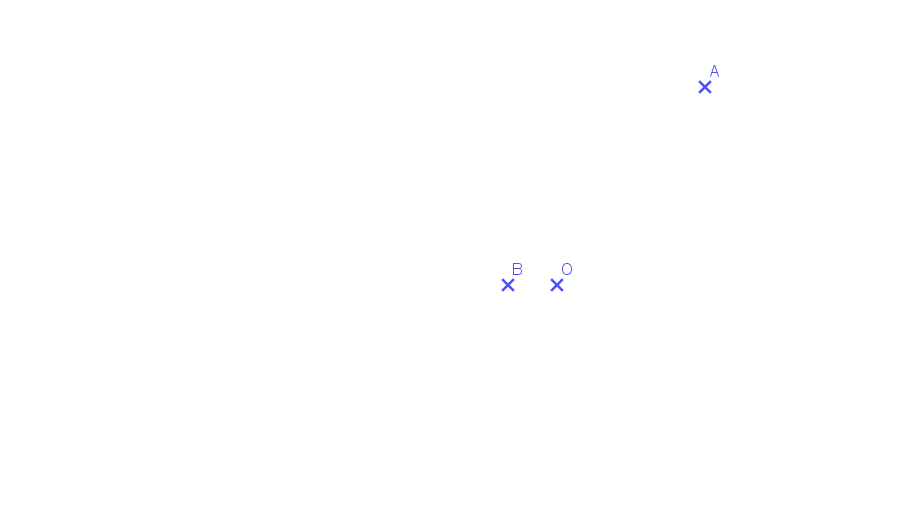
\includegraphics[scale=1]{exohomo1.eps} 

\noindent \initq \q Placer le point B' image du point B par l'homothétie de centre O et de rapport k = 7.\\
\q Placer le point A' image du point A par l'homothétie de centre O et de rapport k = -0,6.\\


\exo{2} Tracer $F_{2}$ l'image de la figure $F_{1}$ par l'homothétie de centre L et de rapport k = 0,5.


\begin{flushleft}
\includegraphics[scale=0.75]{figure1homo.eps} 
\end{flushleft}


\newpage

\exo{3}\\

\initq \q Tracer le polygone C'D'E'F'A'B' l'image du polygone CDEFAB par l'homothétie de  centre G et de rapport $k= \dfrac{1}{3}$ .

\begin{flushleft}
 \includegraphics[scale=0.9]{exohomo2.eps}
 \end{flushleft} 

\q Tracer le polygone A'B'C'D' l'image du polygone ABCD par l'homothétie de  centre E et de rapport $k=- 2$ .

\begin{flushleft}
\includegraphics[scale=0.9]{exohomo3.eps} 
\end{flushleft}

\newpage
\vspace*{1cm}


\exo{2,5}
Soit MONA un rectangle de longueur 12 m et de largeur 5 m et M'O'N'A' son image par une homothétie de rapport k = 6.\\

\noindent \initq \q Calculer l'aire du rectangle MONA.\\
\q Sans tracer de figures et en utilisant une propriété du cours, calculer l'aire du rectangle M'O'N'A'. Quel est le facteur d'agrandissement d'aire ? \textbf{(Justifier votre calcul)}\\

\vspace*{1cm}

 Comprendre l'effet d'une symétrie (axiale et centrale) sur une figure et savoir construire l'image d'une figure par une des symétries 

 Comprendre l'effet d'une translation sur une figure et savoir construire l'image d'une figure par une translation 
 Comprendre l'effet d'une rotation sur une figure et savoir construire l'image d'une figure par une rotation 

Comprendre l'effet d'une homothétie sur une figure et savoir construire l'image d'une figure par une homothétie  


\end{document}
